% ======================= 6. RESULTADOS =======================
\section{Resultados}\label{sec:resultados}

\subsection{Desempeño de M0 y M1}\label{sec:desempeno}

\begin{figure}[!htbp]
\centering
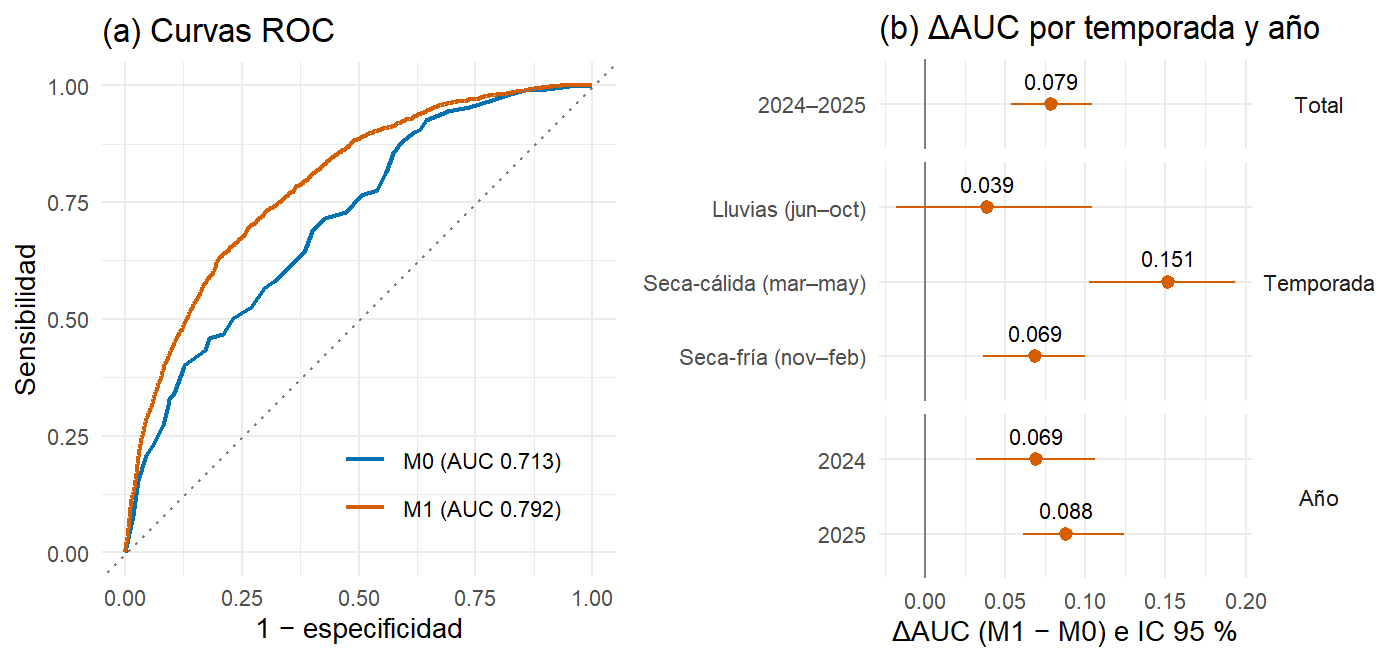
\includegraphics[width=0.64\textwidth]{figuras/roc_y_dauc_informe.png}
\caption{(a) Curvas ROC de M0 y M1 y (b) \dauc{} en total, por temporada y por año, con IC 95\,\% por bootstrap pareado por bloques de 14 días (LDA; prueba 2024–2025, análisis final, n = 6\,863).}
\label{fig:roc}
\end{figure}

\begin{table}[!htbp]
\centering\small
\caption{Desempeño de los dos clasificadores en la prueba 2024–2025 (análisis final, n = 6\,863; 26.2\,\% de superación; corte 0.259). Diferencia M1 − M0 con IC 95\,\% por bootstrap pareado por bloques de 14 días.}
\label{tbl:metricas}
\begin{tabularx}{\textwidth}{>{\raggedright\arraybackslash}p{2.6cm}rrCrrC}
\toprule
Métrica & LDA M0 & LDA M1 & LDA M1 − M0 [IC 95\,\%] & Log. M0 & Log. M1 & Logística M1 − M0 [IC 95\,\%]\\
\midrule
AUC & 0.713 & 0.792 & \textbf{0.079} [0.054, 0.104] & 0.721 & 0.792 & \textbf{0.071} [0.047, 0.095]\\
Exactitud balanceada & 0.634 & 0.711 & 0.077 [0.051, 0.100] & 0.631 & 0.711 & 0.080 [0.054, 0.103]\\
Sensibilidad & 0.565 & 0.742 & 0.177 & 0.580 & 0.739 & 0.158\\
Especificidad & 0.703 & 0.680 & −0.023 & 0.682 & 0.684 & 0.002\\
Puntaje de Brier & 0.172 & 0.154 & −0.018 & 0.170 & 0.153 & −0.017\\
\bottomrule
\end{tabularx}
\end{table}

\textbf{La meteorología del día mejora el AUC entre 0.071 (regresión logística) y 0.079 (LDA) sobre estación y temporada, en la clasificación retrospectiva de 2024–2025} (Tabla~\ref{tbl:metricas}). Estación y temporada ya separan buena parte de los días con superación (AUC de 0.713 con LDA y 0.721 con logística); con la meteorología, los dos llegan a 0.792, y ningún intervalo de la diferencia incluye el cero. M1 detecta el 74\,\% de los días con superación, contra el 56\,\% (LDA) o el 58\,\% (logística) de M0, con una especificidad parecida (LDA: de 0.70 a 0.68; logística: 0.68 en los dos), y el Brier baja. La curva ROC de M1 queda por encima de la de M0 en casi todo el rango (Figura~\ref{fig:roc}, panel a).

\textbf{Por temporada (Figura~\ref{fig:roc}, panel b).} La mejora sobre M0 es mayor en seca-cálida, de marzo a mayo (\dauc{} 0.151 [0.102, 0.193]). En esa temporada la estación separa poco los días (AUC de M0 de 0.58, frente a 0.67–0.68 en las otras dos), así que la meteorología tiene más espacio para aportar. En seca-fría la mejora es de 0.069 [0.037, 0.100]. En la temporada de lluvias es 0.039 (IC 95\,\% [−0.018, 0.104]); este intervalo no permite establecer una ganancia adicional respecto de M0. En esa temporada la superación ocurre en el 9.7\,\% de los días, y el resultado no demuestra ausencia de capacidad discriminante: el AUC de M1 es aproximadamente 0.706. El orden entre temporadas es descriptivo y se refiere a la mejora sobre M0; frente a la persistencia el orden cambia (Sección~\ref{sec:persistencia}). \textbf{Por año}, la mejora es de 0.069 [0.032, 0.106] en 2024 y de 0.088 [0.061, 0.124] en 2025.

\textbf{Días-estación y episodios.} Un episodio es una racha de días consecutivos con superación en una estación; un día sin dato la corta. Los 1\,799 días-estación con superación de la prueba forman 733 episodios (mediana de 2 días y máximo de 16; el 47\,\% dura un solo día). M1 marca al menos un día del 72\,\% de los episodios y el primer día del 66\,\% (M0: 49\,\% en los dos casos); de las 219 rachas que forman los 349 días-estación con PM2.5 > 40\ugm, marca al menos un día del 90\,\% (M0: 77\,\%). Según la magnitud (Figura~\ref{fig:magnitud}, Anexo~C), M1 marca el 90\,\% de los días-estación con PM2.5 > 40\ugm{} (M0: 81\,\%) y el 21\,\% de los que tienen menos de 15\ugm{} (M0: 27\,\%); los errores se concentran cerca de 25\ugm.

\subsection{Estructura de la meteorología (PCA)}\label{sec:pca}
La Figura~\ref{fig:pca} muestra las cargas de los tres componentes, que juntos resumen el 66.5\,\% de la variación de las ocho variables meteorológicas (no de las superaciones). El primero (36\,\%) es un \textbf{día cálido, soleado y ventilado}, con temperatura, radiación y rapidez del viento positivas, y presión y \emph{u} negativas (más flujo del este). El segundo (17\,\%) es un \textbf{día húmedo y lluvioso}, con humedad, lluvia y \emph{v} positivas y \emph{u} negativa. El tercero (13\,\%) es un \textbf{día de presión baja y poco viento}.

\begin{figure}[!htbp]
\centering
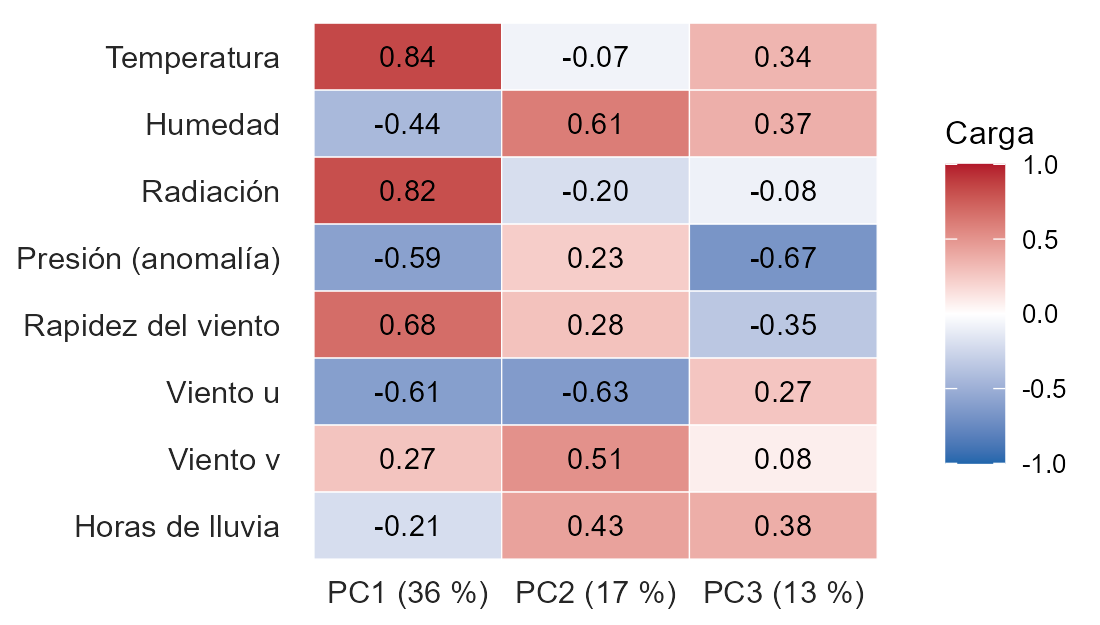
\includegraphics[width=0.46\textwidth]{figuras/pca_cargas_informe.png}
\caption{Cargas de los tres primeros componentes principales (anomalías por estación; entrenamiento 2021–2023 del análisis final, n = 10\,965). Entre paréntesis, el porcentaje de varianza de las ocho variables meteorológicas que explica cada componente.}
\label{fig:pca}
\end{figure}

\subsection{Coeficientes del LDA y de la logística}\label{sec:coef}
Solo interpretamos los coeficientes cuyo signo se mantiene en al menos el 95\,\% de 1\,000 réplicas del bootstrap por bloques en el entrenamiento (Figura~\ref{fig:coef}). Con signo estable, y condicional a las demás variables, la superación se asocia con \textbf{menor rapidez del viento} (−0.50 [−0.63, −0.35]), \textbf{presión más baja de lo normal para el sitio} (−0.46 [−0.57, −0.30]) y \textbf{mayor temperatura} (0.44 [0.16, 0.70]), y en menor medida con menos horas de lluvia y menos radiación. La temperatura tiene una correlación de estructura casi nula (−0.07), es decir, poca correlación marginal con el puntaje discriminante, aunque su coeficiente es positivo al ajustar por estación, temporada y las demás variables; estas correlaciones no sustituyen a los coeficientes condicionales (Rencher, 1992), y no interpretamos ese coeficiente común como una demostración separada para cada temporada. Por eso el primer componente, que junta temperatura y viento, mezcla efectos opuestos. Las ocho variables meteorológicas tienen el mismo signo en el LDA y en la logística (panel b; Sección~\ref{sec:logistica}), y las cinco de signo estable lo conservan en los pliegues que validan 2022 y 2023. \textbf{No interpretamos la humedad ni las componentes \emph{u} y \emph{v},} cuyo signo no es estable, ni ordenamos las variables por el tamaño de su coeficiente.

Dos signos piden cautela. \textbf{Radiación:} sin ajustar, dentro de cada temporada, se asocia ligeramente con más superación (correlación de +0.06 a +0.11), y el signo negativo solo aparece al ajustar; además, las partículas reducen la radiación que llega a la superficie, así que la relación puede ir del PM2.5 a la radiación, y no la interpretamos como efecto. \textbf{Presión:} la asociación con presión baja aparece también sin ajustar dentro de cada temporada (correlación de −0.20 a −0.30), así que no es un artefacto del modelo, pero va en contra de la explicación más común, que liga la acumulación con sistemas de alta presión. En nuestros datos la anomalía de presión baja acompaña al aire más cálido (correlación de −0.52 a −0.68 con la temperatura), y una explicación posible son situaciones previas al paso de frentes; es una hipótesis sin respaldo en este análisis, que requiere datos sinópticos.

\begin{figure}[!htbp]
\centering
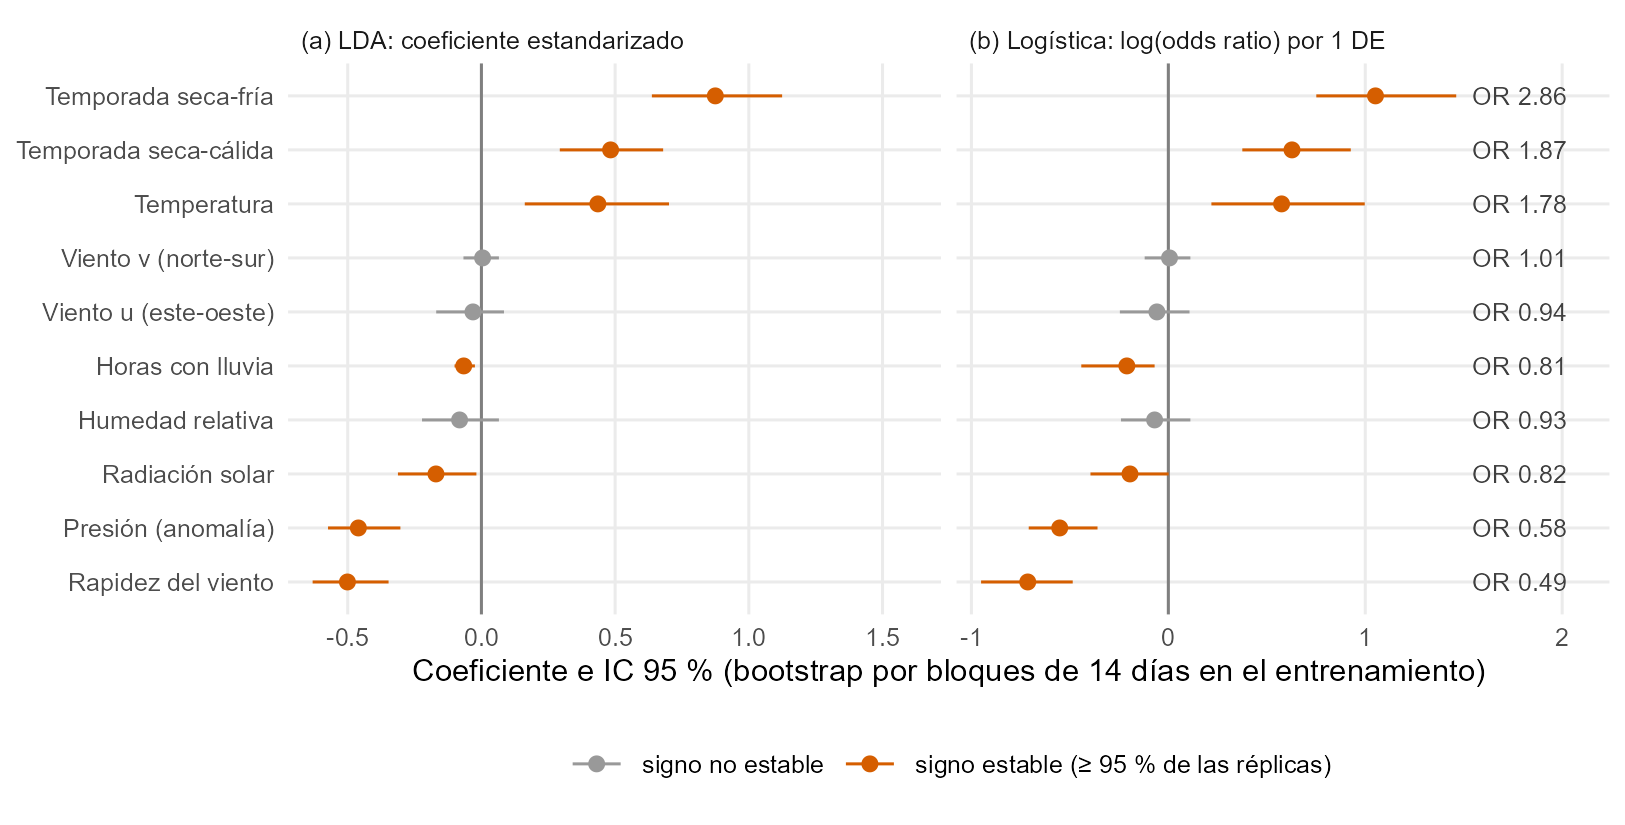
\includegraphics[width=0.68\textwidth]{figuras/coef_lda_logistica_informe.png}
\caption{Coeficientes de la meteorología y la temporada en M1: (a) LDA, coeficiente estandarizado; (b) regresión logística, logaritmo del odds ratio (OR) por 1 DE, con el OR a la derecha. IC 95\,\% por bootstrap por bloques de 14 días en el entrenamiento (1\,000 réplicas, n = 10\,965). En color, los de signo estable; la radiación lo es, pero su intervalo en la logística llega a 1, así que su efecto es débil. Las indicadoras de estación están en el Anexo~C.}
\label{fig:coef}
\end{figure}

\subsection{Robustez y sensibilidades}\label{sec:robustez}
La mejora se mantiene entre 0.071 y 0.082 en todas las variantes de preparación y validación, y ningún intervalo incluye el cero (Tabla~\ref{tbl:robustez}, Anexo~C): logística, MICE (0.078), bloques de 7 y 28 días, otras definiciones de la respuesta y de las reubicaciones, radiación no negativa y sin la estación NO2. Con splines, la logística llega a 0.090 (Sección~\ref{sec:logistica}). En la prueba, la mejora es de 0.095 en los días con meteorología completada con la mediana de la red y de 0.074 en los demás; sin imputación diaria, 0.071. La conclusión se conserva con las dos estrategias de imputación diaria comparadas; no se pudo comparar con MIMA-v1 (Sección~\ref{sec:imputacion}).

\subsection{Persistencia frente a meteorología}\label{sec:persistencia}
Como línea base usamos la persistencia: el PM2.5 del día calendario anterior en la misma estación, con al menos 18\,h observadas. Quedan 10\,345 días-estación de entrenamiento y 6\,280 de prueba, con 26.3\,\% de superación en los dos. El logaritmo no mejoró el AUC de validación en los dos pliegues, así que se usa la escala original. La Tabla~\ref{tbl:persistencia} compara M0, M1, MP (M0 más el PM2.5 del día anterior) y MP1 (MP más la meteorología).

\begin{table}[!htbp]
\centering\small
\caption{Persistencia frente a meteorología en la prueba 2024–2025, en los días-estación con PM2.5 del día anterior (n = 6\,280): AUC de cada modelo y diferencias con IC 95\,\% por bootstrap pareado por bloques de 14 días. ‡ Cálculo de verificación con las mismas definiciones (reproduce el total de 0.016 [0.008, 0.025]); solo LDA.}
\label{tbl:persistencia}
\begin{tabularx}{\textwidth}{Lrr}
\toprule
Modelo o diferencia & LDA & Logística\\
\midrule
M0: estación + temporada & 0.712 & 0.720\\
M1: M0 + meteorología del día & 0.792 & 0.792\\
MP: M0 + PM2.5 del día anterior & 0.872 & 0.872\\
MP1: MP + meteorología del día & 0.887 & 0.888\\
M1 − MP: meteorología del día frente a persistencia & −0.080 [−0.103, −0.055] & −0.079 [−0.101, −0.057]\\
MP1 − MP: lo que la meteorología agrega a la persistencia & 0.016 [0.008, 0.025] & 0.016 [0.007, 0.025]\\
\quad seca-fría (nov–feb; n = 2\,179)‡ & 0.036 [0.020, 0.053] & —\\
\quad seca-cálida (mar–may; n = 1\,571)‡ & 0.018 [0.001, 0.033] & —\\
\quad lluvias (jun–oct; n = 2\,530)‡ & 0.002 [−0.013, 0.020] & —\\
M1 − M0 en esta submuestra & 0.079 [0.054, 0.106] & 0.072 [0.048, 0.098]\\
\bottomrule
\end{tabularx}
\end{table}

\textbf{La persistencia clasifica mejor que la meteorología del día:} M1 queda 0.080 por debajo de MP (IC 95\,\% [−0.103, −0.055]) con los dos clasificadores. Sobre la persistencia, la meteorología agrega poco, aunque su intervalo no incluye el cero: MP1 − MP = 0.016 [0.008, 0.025]. \textbf{El orden por temporada depende de la base de comparación:} frente a M0 la meteorología aporta más de marzo a mayo, pero frente a la persistencia aporta más de noviembre a febrero (0.036) y nada distinguible de cero en lluvias. \textbf{La comparación sigue siendo retrospectiva:} el PM2.5 del día anterior estaría disponible antes del día evaluado y la meteorología observada del mismo día no; no es una prueba de pronóstico.

\subsection{Umbral de clasificación}\label{sec:umbral}
El corte actual (0.259, la prevalencia del entrenamiento) equilibra sensibilidad y especificidad, pero un uso operativo debe elegirlo según su objetivo. Lo elegimos sin usar la prueba, con las predicciones fuera de muestra de los pliegues de 2022 y 2023: \textbf{vigilancia}, el corte más alto con sensibilidad ≥ 0.80, para limitar los falsos negativos, y \textbf{equilibrio}, el que maximiza el índice de Youden (sensibilidad + especificidad − 1; Youden, 1950). La Tabla~\ref{tbl:umbral} da su desempeño en la prueba, y la Figura~\ref{fig:cortes} (Anexo~C), las métricas con cortes de 0.10 a 0.60.

\begin{table}[!htbp]
\centering\small
\caption{Cortes de clasificación de M1 elegidos sin usar la prueba (predicciones de los pliegues de 2022 y 2023) y su desempeño en la prueba 2024–2025 (n = 6\,863). VPP: valor predictivo positivo; FA: falsas alarmas por cada superación detectada; \% marcados: días clasificados como superación.}
\label{tbl:umbral}
\begin{tabularx}{\textwidth}{lLrrrrrrr}
\toprule
Clasificador & Objetivo & Corte & Sensib. & Especif. & VPP & FA & Exact. bal. & \% marcados\\
\midrule
LDA & Vigilancia (sensibilidad ≥ 0.80) & 0.182 & 0.839 & 0.566 & 0.407 & 1.46 & 0.702 & 54.0\\
LDA & Equilibrio (Youden) & 0.262 & 0.738 & 0.684 & 0.454 & 1.20 & 0.711 & 42.6\\
LDA & Actual (prevalencia) & 0.259 & 0.742 & 0.680 & 0.451 & 1.22 & 0.711 & 43.1\\
Logística & Vigilancia (sensibilidad ≥ 0.80) & 0.192 & 0.826 & 0.585 & 0.414 & 1.41 & 0.705 & 52.3\\
Logística & Equilibrio (Youden) & 0.267 & 0.727 & 0.695 & 0.459 & 1.18 & 0.711 & 41.5\\
Logística & Actual (prevalencia) & 0.259 & 0.739 & 0.684 & 0.454 & 1.20 & 0.711 & 42.7\\
\bottomrule
\end{tabularx}
\end{table}

Con el corte de vigilancia (0.182 en el LDA), M1 detecta el 84\,\% de las superaciones de la prueba, pero marca el 54\,\% de los días y da 1.46 falsas alarmas por detección; con el de equilibrio (0.262, casi el actual), detecta el 74\,\% con 1.20. La exactitud balanceada casi no cambia (0.70–0.71): la elección depende del costo que SIMA asigne a una superación no detectada frente a una falsa alarma. Recomendamos el de vigilancia para no perder superaciones y el de equilibrio para limitar las falsas alarmas. Las probabilidades no están calibradas (pendiente 0.82; Sección~\ref{sec:errores}): el corte es un umbral sobre un puntaje, no un riesgo, y habría que revisarlo si se recalibra el modelo o se usa meteorología pronosticada.

% ======================= 7. DISCUSIÓN =======================
\section{Discusión y conclusiones}\label{sec:conclusiones}

\textbf{Conclusión.} La meteorología del día mejora el AUC entre 0.071 (regresión logística) y 0.079 (LDA) sobre estación y temporada, en la clasificación retrospectiva de 2024–2025, y la detección de superaciones pasa de 56–58\,\% a 74\,\%. La conclusión se limita al periodo evaluado: \textbf{no se respalda un pronóstico.}

\textbf{Hallazgos.} Como señaló SIMA, el PM2.5 no tiene una periodicidad tan marcada como la del ozono (comunicación personal, 15 de octubre de 2026); por eso estación y temporada separan solo una parte de los días. Frente a M0, la mejora es mayor de marzo a mayo, donde la estación separa peor; es estable en dos años de prueba, en la validación progresiva y en las variantes analizadas, y sube a 0.090 con relaciones no lineales. Con los dos clasificadores, las superaciones se asocian con viento débil, presión más baja de lo normal y, al ajustar por estación y temporada, mayor temperatura. El viento débil es coherente con la acumulación de partículas con poca ventilación documentada en la ZMM (Martínez-Cinco et al., 2016) y con la persistencia de las excedencias en la temporada seca (Hernández-Romero et al., 2026); la presión baja va contra la explicación más común y queda como hipótesis por verificar (Sección~\ref{sec:coef}). \textbf{Frente a la persistencia, la meteorología del día no basta:} el PM2.5 del día anterior clasifica mejor (AUC 0.872 frente a 0.792) y la meteorología le agrega 0.016, sobre todo de noviembre a febrero, así que un aviso debería partir de la persistencia. La Tabla~\ref{tbl:concluir} delimita las conclusiones.

\begin{table}[!htbp]
\centering\small
\caption{Qué permite concluir este análisis y qué no.}
\label{tbl:concluir}
\begin{tabularx}{\textwidth}{LL}
\toprule
Sí se puede concluir & No se puede concluir\\
\midrule
Que una combinación lineal de estación, temporada y meteorología separa los días con y sin superación fuera de muestra (AUC 0.792 en 2024–2025) & Causas: es un estudio observacional y el modelo encuentra asociaciones\\
Cuánto añade la meteorología sobre estación y temporada: \dauc{} de 0.071 (logística) a 0.079 (LDA), con la misma partición & Qué variable es más importante, ni por el tamaño de su coeficiente ni por permutación, ni la significancia de cada coeficiente (los datos son dependientes)\\
La dirección de la asociación condicional de las variables de signo estable: viento, presión, temperatura y lluvia; la radiación, con un efecto débil y posiblemente invertido & Probabilidades exactas: no están calibradas (pendiente 0.82)\\
Que, frente a M0, la mejora es mayor de marzo a mayo y no se distingue de cero en lluvias (descriptivo) & Capacidad de pronóstico: usa meteorología observada del mismo día\\
Que la persistencia clasifica mejor que la meteorología del día, que le agrega poco (0.016) & Que sea una alerta operativa o un modelo temporal: la dependencia se acota, no se modela\\
\bottomrule
\end{tabularx}
\end{table}

\textbf{Limitaciones.} (1) Es retrospectivo: una alerta necesita meteorología pronosticada, cuyo error reduciría la mejora; lo mismo aplica a la aplicación Shiny del repositorio, que muestra esta evaluación retrospectiva. (2) La prueba ya se había usado (Sección~\ref{sec:supuestos}), los pliegues internos no repiten la imputación (Sección~\ref{sec:validacion}) y las Secciones~\ref{sec:logistica}, \ref{sec:persistencia} y~\ref{sec:umbral} son posteriores a la evaluación. (3) La dependencia entre días y estaciones que el modelo no absorbe impide interpretar errores estándar: \textbf{las medidas tomadas acotan la incertidumbre y evalúan el desempeño, pero no convierten el análisis en un modelo temporal completo ni en una alerta operativa.} (4) La muestra no es aleatoria, y los días sin PM2.5 se concentran en NO (57\,\%), NE2 (33\,\%) y SUR (26\,\%) y en 2024–2025 (Sección~\ref{sec:muestra}); el 27\,\% de los días de prueba tiene meteorología completada con la red. (5) Hubo cambios de equipos, reubicaciones y una anomalía del PM2.5 de NO2: la mitad de sus días de prueba caen en ese periodo (272 días, sin ninguna superación); las sensibilidades no cambian la conclusión, pero faltan fechas confirmadas. (6) No hay altura de capa de mezcla ni información de emisiones. (7) La forma lineal es una aproximación (Sección~\ref{sec:logistica}), las probabilidades no están calibradas y los cortes son únicos para toda la red (Anexo~C).

\textbf{Recomendaciones para SIMA, por prioridad.} (1) Evaluar el modelo con meteorología pronosticada y con la persistencia como base, con su área de pronósticos. (2) Elegir el corte según el uso (Sección~\ref{sec:umbral}): 0.18 para vigilancia o 0.26 para limitar las falsas alarmas; después, definir cortes por estación y recalibrar las probabilidades antes de comunicarlas. (3) Incorporar a su control de calidad las reglas de radiación de madrugada y de viento contra la red. (4) Revisar los sensores de radiación de NO2 y NTE y el equipo de PM2.5 de NO2 entre 2023 y 2025. (5) Hacer un análisis horario de transporte en Santa Catarina (SO) y Juárez (SE2).

\textbf{Preguntas nuevas.} ¿Se sostiene la mejora en una evaluación de pronóstico, con meteorología pronosticada? ¿Cambia la conclusión con un modelo temporal explícito (errores autocorrelacionados o efectos aleatorios por estación)? ¿En Santa Catarina domina el transporte desde la ciudad o la acumulación local? ¿Qué papel tienen la fracción gruesa y la resuspensión en Juárez? ¿Qué efecto tuvieron la política ambiental de 2022 y la pandemia? ¿Hay grupos de estaciones con una sensibilidad meteorológica parecida? ¿Cambia la mejora si la meteorología se completa con la reconstrucción de MIMA-v1?
